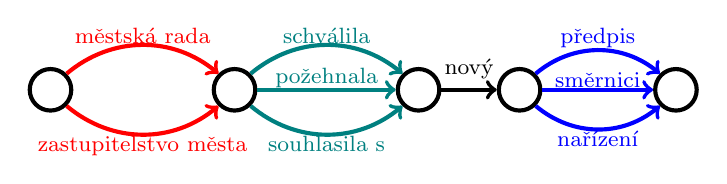
\begin{tikzpicture}	
	\tikzstyle{unit} = [circle,line width=1.5pt,draw,minimum size=1.5em]
		
		\node[unit] (u1)at (0,0){};
		\node[unit,anchor=west](u2) at ([xshift=5em]u1.east){};
		\node[unit,anchor=west](u3) at ([xshift=5em]u2.east){};
		\node[unit,anchor=west](u4) at ([xshift=2em]u3.east){};
		\node[unit,anchor=west](u5) at ([xshift=4em]u4.east){};
		
		\draw[->,out=40,in=140,red,line width=1.5pt] (u1.north east) to  node[inner sep=0pt,color=red,above]{\footnotesize městská rada}(u2.north west);
		\draw[->,out=-40,in=-140,red,line width=1.5pt] (u1.south east) to  node[inner sep=0pt,color=red,below]{\footnotesize zastupitelstvo města}(u2.south west);
		
		\draw[->,out=40,in=140,teal,line width=1.5pt] (u2.north east) to  node[inner sep=0pt,color=teal,above]{\footnotesize schválila}(u3.north west);
		\draw[->,teal,line width=1.5pt](u2.east)-- node[inner sep=0pt,color=teal,above]{\footnotesize požehnala}(u3.west);
		\draw[->,out=-40,in=-140,teal,line width=1.5pt] (u2.south east) to  node[inner sep=0pt,color=teal,below]{\footnotesize souhlasila s}(u3.south west);
		\draw[->,line width=1.5pt](u3.east) -- node[above]{\footnotesize nový} (u4.west);
		
		\draw[->,out=40,in=140,blue,line width=1.5pt] (u4.north east) to  node[inner sep=0pt,color=blue,above]{\footnotesize předpis}(u5.north west);
		\draw[->,blue,line width=1.5pt](u4.east)-- node[inner sep=0pt,color=blue,above]{\footnotesize směrnici}(u5.west);
		\draw[->,out=-40,in=-140,blue,line width=1.5pt] (u4.south east) to  node[inner sep=0pt,color=blue,below]{\footnotesize nařízení}(u5.south west);
		
\end{tikzpicture}
